\documentclass[../main.tex]{subfiles}
\begin{document}
\chapter{Numerical Sequences and Series}
\section{Sequences}
\begin{definition}[Sequence]
  A \textit{sequence} $(x_n)_{n \in \N}$ on a set $X$ is an enumerated list (i.e. $x_1, x_2, x_3, \ldots$) where each element is in $X$.
\end{definition}
In this chapter, we will consider only sequences where $X \subseteq \R$ or $X \subseteq \C$.
A concrete and important example is $X = \R$ which are known as the \textit{real sequences}.

\subsection{Convergence and Divergence}
We would like to think about what it means for a sequence $x_n$ to converge to a point $x \in X$, and what it means for $x_n$ to diverge to infinity?

\textbf{On convergence}
\begin{itemize}
  \item We need $|x_n - x|$ to be small, more specifically, smaller than any given threshold $\varepsilon > 0$ that we choose.
  \item For this comparison, only the ``tail'' of the sequence, i.e. the ``large $n$'' behaviour, matters.
    We can always ignore the first $N$ terms of the sequence, for some $N$ dependent on $\varepsilon$.
\end{itemize}
\textbf{On divergence to infinity}
\begin{itemize}
  \item We need $|x_n|$ to clear any threshold $L > 0$ that we set for it.
  \item Again, only the ``tail'' matters.
    We can always ignore the first $N$ terms, for some $N$ dependent on $L$.
\end{itemize}
Now that we know what we what restrictions we want the definitions to impose, we can more rigorously state them:
\begin{definition}[Convergence]
  We say that the sequence $(x_n)$ \textit{converges} to some finite $x \in \C$ if:
  \[
    \forall \varepsilon > 0\ \exists N = N(\varepsilon) \text{ s.t. } |x_n - x| < \varepsilon\ \forall n \geq N
  \]
  We then write $x_n \to x$.
\end{definition}
\begin{definition}[Divergence to infinity]
  We say that the sequence $(x_n)$ \textit{diverges to infinity} if $\frac{x_n}{|x_n|}$ converges and:
  \[
    \forall L > 0\ \exists N = N(L) \text{ s.t. } |x_n| > L\ \forall n \geq N
  \]
\end{definition}
\begin{remark}[Remarks]
  \begin{enumerate}
    \item We can make the modulus inequality non strict (i.e. $|x_n - x| \leq \varepsilon$ for convergence or $|x_n| \geq L$ for divergence to infinity) for an equivalent definition.
    \item We can also replace $\varepsilon$ by any constant positive multiple of $\varepsilon$ for an equivalent definition.
    \item For divergence to infinity, we require that $\frac{x_n}{|x_n|}$ converges so that for a complex sequence, it diverges in a specific direction.
      This excludes cases where the sequence could spiral outwards with increasing modulus.
    \item If $(x_n)$ is real, then it diverges to infinity if either $(x_n)$ or $(-x_n)$ satisfy:
      \[
        \forall L > 0\ \exists N = N(L) \text{ s.t. } x_n > L\ \forall n \geq N
      \]
  \end{enumerate}
\end{remark}
\begin{definition}[Floor and Ceiling functions]
  The \textit{floor function} takes as input any $x \in \R$ and outputs the \textbf{greatest integer less than or equal} to $x$.
  It is denoted $\floor{x}$.

  Similarly, the \textit{ceiling function} takes as input any $x \in \R$ and outputs the \textbf{greatest integer greater than or equal} to $x$.
  It is denoted $\ceil{x}$.
\end{definition}
\begin{example}
  \begin{enumerate}
    \item $x_n = \frac{1}{n}$, then $x_n \to 0$ as $\forall \varepsilon > 0$, we have:
      \[
        |x_n - 0| = \frac{1}{n} < \varepsilon\ \forall n \geq N = N(\varepsilon) = 1 + \ceil{\frac{1}{\varepsilon}}
      \]
    \item $x_n = \frac{1}{2^{n}}$ then $x_n \to 0$ as $\forall \varepsilon > 0$, we have:
      \[
        |x_n - 0| = \frac{1}{2^{n}} < \varepsilon\ \forall n \geq N = N(\varepsilon) = \max\left\{1 + \log_2\left(\frac{1}{\varepsilon}\right), 1\right\}
      \]
      Note that we use the $\max$ to avoid issues when $\log_{2}(1/\varepsilon) < 0$.
    \item $x_n = i n$ diverges to infinity as $\forall L > 0$, we have:
      \[
        \frac{x_n}{i} = n > L\ \forall n \geq N = 1 + \ceil{L}
      \]
    \item $x_n = (-1)^{n}$ does not diverge to $\infty$ (as $|x_n| \leq 1\ \forall n$), but also does not converge (See Numbers and Sets -- Example 6.5).
  \end{enumerate}
\end{example}
\subsection{Limit Laws and Properties}
\begin{lemma}[Uniqueness of Limits]
  If it exists, the limit of $(x_n)$ is unique.
\end{lemma}
\begin{proof}
  Suppose $x_n \to a$ and $x_n \to b$.
  Take $\varepsilon > 0$, we then have:
  \begin{align*}
    \exists N_1 &= N_1(\varepsilon) \text{ s.t. } |x_n - a| < \varepsilon\ \forall n \geq N_1 \\
    \exists N_2 &= N_2(\varepsilon) \text{ s.t. } |x_n - b| < \varepsilon\ \forall n \geq N_2
  \end{align*}
  In particular $|x_n - a|, |x_n - b| < \varepsilon\ \forall n \geq N = \max\{N_1, N_2\}$, thus, using the triangle inequality:
  \[
    |a - b| = |a - x_n + x_n - b| \leq |x_n - a| + |x_n - b| < 2\varepsilon\ \forall n \geq N
  \]
  Now since $\varepsilon$ can be arbitrarily small and positive, we conclude that $|a - b| = 0$ and so $a = b$.
\end{proof}
\begin{remark}[Notation]
  Since the limit is unique, we write:
  \[
    \lim_{n \to \infty} x_n = x
  \]
  to mean the unique limit of $x_n$ as $n \to \infty$.
\end{remark}
\begin{proposition}[Sandwich Theorems]
  Let $(x_n), (y_n), (z_n)$ be real sequences.
  \label{sandwichThm}
  Then:
  \begin{enumerate}
    \item If $x_n \leq y\ \forall n$ and $x_n \to x$, then $x \leq y$
    \item If $x_n \to x$, $z_n \to x$ and $x_n \leq y_n \leq z_n\ \forall n$, then $y_n \to x$ also.
  \end{enumerate}
\end{proposition}
\begin{proof}[\textbf{i}]
  Suppose, for contradiction, that $x > y$.
  Then $x - y > 0$, so we can take $\varepsilon = x - y$.
  Thus $\exists N \text{ s.t. } |x_n - x| < x - y \ \forall n \geq N$.
  However, $x_n \leq y < x$ so:
  \[
    |x_n - x| = x - x_n < x - y \implies x_n > y\ \forall n \geq N
  \]
  which is a contradiction.
\end{proof}
\begin{proof}[\textbf{ii}]
  Take $\varepsilon > 0$, we then have:
  \begin{align*}
    \exists N_1 &= N_1(\varepsilon) \text{ s.t. } |x_n - a| < \varepsilon\ \forall n \geq N_1 \\
    \exists N_2 &= N_2(\varepsilon) \text{ s.t. } |x_n - b| < \varepsilon\ \forall n \geq N_2
  \end{align*}
  We can then write:
  \begin{align*}
    |y_n - x| &= \frac{1}{2}|(x_n - x) + (z_n - x) + (y_n - x_n) + (y_n - z_n)| \\
              &< \frac{1}{2}(2\varepsilon + |y_n - x_n| + |y_n - z_n|) \\
              &= \frac{1}{2}(2\varepsilon + y_n - x_n + z_n - y_n) \\
              &= \varepsilon + \frac{1}{2}(z_n - x_n) \\
              &= \varepsilon + \frac{1}{2}|z_n - x_n| \\
              &\leq \varepsilon + \frac{1}{2}(|z_n - x| + |x_n - x|) \\
              &< 2\varepsilon
  \end{align*}
  So $y_n \to x$.
\end{proof}
\begin{remark}
  Note that $x_n < y\ \forall n$ and $x_n \to x$ does not necessarily imply $x < y$.

  For example, $x_n = 1 - \frac{1}{n} < 1\ \forall n$ but $x_n \to 1$.
\end{remark}
\begin{lemma}
  Let $(x_n)$ be a complex sequence.
  Then $x_n \to x$ if and only if $\Re(x_n) \to \Re(x)$ and $\Im(x_n) \to \Im(x)$.
  \label{complexConvergence}
\end{lemma}
\begin{proof}
  Recall that for $z \in \C$, $|z| = \sqrt{(\Re(z))^2 + (\Im(z))^2}$.
  \begin{proofdirection}{Assume $x_n \to x$}
    If we fix $\varepsilon > 0$, by definition of convergence:
    \[
      \exists N \text{ s.t } |x_n - x| < \varepsilon\ \forall n \geq N
    \]
    We see that $|\Re(z)| \leq |z|$ and $|\Im(z)| \leq |z|$.
    Therefore for all $n \geq N$:
    \begin{align*}
      |\Re(x_n) - \Re(x)| &= |\Re(x_n - x)| \leq |x_n - x| < \varepsilon \\
      |\Im(x_n) - \Im(x)| &= |\Im(x_n - x)| \leq |x_n - x| < \varepsilon
    \end{align*}
    So $\Re(x_n) \to \Re(x)$ and $\Im(x_n) \to \Im(x)$.
  \end{proofdirection}
  \begin{proofdirection}{Assume $\Re(x_n) \to \Re(x)$ and $\Im(x_n) \to \Im(x)$}
    If we fix $\varepsilon > 0$, by definition of convergence:
    \begin{align*}
      \exists N_1 &= N_1(\varepsilon) \text{ s.t. } |\Re(x_n) - \Re(x)| < \varepsilon\ \forall n \geq N_1 \\
      \exists N_2 &= N_2(\varepsilon) \text{ s.t. } |\Im(x_n) - \Im(x)| < \varepsilon\ \forall n \geq N_2
    \end{align*}
    We see that:
    \[
      |z| = |\Re(z) + i \Im(z)| \leq |\Re(z)| + |i||\Im(z)| = |\Re(z)| + |\Im(z)|
    \]
    and so:
    \[
      |x_n - x| \leq |\Re(x_n) - \Re(x)| + |\Im(x_n) - \Im(x)| < 2\varepsilon\ \forall n \geq \max\{N_1, N_2\}
    \]
  \end{proofdirection}
\end{proof}
\begin{definition}[Bounded Sequence]
  We say that $(x_n)$ is bounded if $\exists M > 0$ such that $|x_n| \leq M$ or equivalently $\sup\limits_{n \geq 1} |x_n| \leq M$.
\end{definition}
\begin{lemma}[Boundedness of Convergent Sequences]
  If $x_n \to x$ then $(x_n)$ must be bounded.
  That is $\exists M$ s.t. $|x_n| \leq M\ \forall n$.
  \label{convergenceBounded}
\end{lemma}
\begin{proof}
  Take $\varepsilon = 1$, then $\exists N \text{ s.t. } |x_n - x| \leq 1\ \forall n \geq N$ and thus by the triangle inequality:
  \[
    |x_n|  = |x_n - x + x| \leq |x_n - x| + |x| \leq 1 + |x|\ \forall n \geq N
  \]
  For $n < N$, $|x_n| \leq \max\{|x_1|, \ldots, |x_{N - 1}|\} < \infty$

  Therefore the whole sequence is bounded by:
  \[
    |x_n| \leq \max\{|x_1|, \ldots, |x_{N - 1}|, 1 + |x|\}\ \forall n
  \]
\end{proof}
\begin{lemma}[Addition and Multiplication of Limits]
  If $x_n \to x$ and $y_n \to y$, then:
  \label{limitLaws}
  \begin{enumerate}
    \item $x_n + y_n \to x + y$
    \item $x_n y_n \to xy$
  \end{enumerate}
\end{lemma}
\begin{proof}
  Since $x_n \to x$ and $y_n \to y$, $\forall \varepsilon > 0\ \exists N_1 = N_1 (\varepsilon),\ N_2 = N_2(\varepsilon)$ such that:
  \[
    |x_n - x| < \varepsilon\ \forall n \geq N_1 \text{ and } |y_n - y| < \varepsilon\ \forall n \geq N_2
  \]

  \textbf{Addition of Limits (i):}
  \[
    |x_n + y_n - (x + y)| \leq |x_n - x| + |y_n - y| < 2\varepsilon\ \forall n \geq \max\{N_1, N_2\}
  \]
  which is a constant multiple of $\varepsilon$, so we are done.

  \textbf{Multiplication of Limits (ii):}
  \begin{align*}
    |x_n y_n - xy| &= |x_n y_n - xy_n + xy_n - xy| \\
                   &= |x| |y_n - y| + |y_n||x - x_n|
  \end{align*}
  Hence $|x_n y_n - xy| \leq \varepsilon(|x| + |y_n|)\ \forall n \geq \max\{N_1, N_2\}$.
  By \cref{convergenceBounded}, for some $M \geq 0$, we have:
  \[
    |x_ny_n - xy| \leq \varepsilon(|x| + |y_n|) \leq \varepsilon(|x| + M)\ \forall n \geq \max\{N_1, N_2\}
  \]
  which is a constant multiple of $\varepsilon$, so we are done.
\end{proof}
\begin{lemma}[Convergence of Reciprocal Sequence]
  If $x_n \neq 0\ \forall n$ and $x_n \to x \neq 0$, then $\frac{1}{x_n} \to \frac{1}{x}$
  \label{reciprocalConvergence}
\end{lemma}
\begin{proof}
  Since $x_n \to x$ and $x \neq 0$, we can take $\varepsilon = |x/2|$ so $\exists N$ s.t. $|x_n - x| < |x/2|\ \forall n \geq N$.
  Using the triangle inequality, for such $n$ we have:
  \[
    |x_n - (x_n - x)| \leq |x_n| + |x_n - x| \implies |x_n| \geq |x| - |x_n - x| > |x| - \abs{\frac{x}{2}} = \abs{\frac{x}{2}}
  \]
  Since there are finitely many terms with index $< N$, we can construct the bound:
  \[
    |x_n| \geq \min\{|x_1|, \ldots, |x_{N - 1}|, |x/2|\}\ \forall n
  \]
  So $|x_n| \geq M\ \forall n$ for some $M > 0$.

  Now for any $\varepsilon > 0$, $\exists N(\varepsilon)$ s.t. $\forall n > N$ we have the following:
  \begin{align*}
    \abs{\frac{1}{x_n} - \frac{1}{x}} &= \abs{\frac{x_n - x}{x_n x}} \\
                                      &< \frac{\varepsilon}{|x_n||x|} \\
                                      &\leq \frac{\varepsilon}{M|x|}
  \end{align*}
  which is a constant multiple of $\varepsilon$, so we are done.
\end{proof}
\begin{remark}
  This proof also shows that if $x_n \neq 0\ \forall n$ and $x_n \to x \neq 0$, then $\exists M > 0$ such that $|x_n| \geq M\ \forall n$.
\end{remark}
\begin{remark}[Advice]
  We often specify that something must be true for all terms of the sequence, however if it is not, we can just define a new sequence that removes terms from the start of the sequence so that the property is satisfied for all $n$.
\end{remark}
\subsection{Monotone Sequences}
\begin{definition}[Monotone Sequence]
  We say a real sequence $(x_n)$ is \textit{monotone} if either:
  \begin{itemize}
    \item It is \textit{increasing} $x_n \leq x_{n + 1}\ \forall n$ (strictly increasing if $<$)
    \item It is \textit{decreasing} $x_n \geq x_{n + 1}\ \forall n$ (strictly decreasing if $>$)
  \end{itemize}
\end{definition}
\begin{proposition}[Monotone Convergence Theorem]
  Every bounded monotone real sequence converges.
  \label{monotoneConvergence}
\end{proposition}
\begin{proof}
  Suppose $(x_n)$ is increasing.
  Then the set $\{x_n: n \geq 1\}$ is a non-empty set which is bounded above as $(x_n)$ is bounded.
  By the least upper bound axiom, it has a supremum, say $\ell$.

  Given $\varepsilon > 0$, $\ell - \varepsilon$ cannot be an upper bound for the set because $\ell$ is the least upper bound.
  Therefore $\exists N$ s.t. $x_N > \ell - \varepsilon$.
  Thus, since $(x_n)$ is monotonic $\ell - \varepsilon < x_n \leq \ell$ for $\forall n \geq N$.
  Hence $\forall n \geq N$, $|x_n -\ell| < \varepsilon$ so $x_n \to \ell$.

  The decreasing case is the same but instead considering $(-x_n)$.
\end{proof}
\begin{remark}
  We only required the sequence to be bounded above if it is monotonically increasing and bounded below if it is monotonically decreasing.
\end{remark}
Sequences that are bounded but not monotone do not necessarily have to converge, for example the sequence $x_n = (-1)^{n}$ is bounded but does not converge.
However, if we remove even terms we get the subsequence $x_{2k + 1} = -1$, and if we remove all the odd terms, we get the subsequence $x_{2k} = 1$.
These are constant sequences so converge.
\section{Bolzano-Weierstrass Theorem}
To prove the Bolzano-Weierstrass Theorem, we first need to rigorously introduce the notion of a subsequence and prove a few preliminary lemmas.
\begin{definition}[Subsequence]
  Given a sequence $(x_n)$, a \textit{subsequence} of $(x_n)$ is a sequence of the form $(x_{n_k})_{k \in \N}$ where $(n_k)_{k \in \N}$ is a sequence of naturals satisfying $n_1 < n_2 < n_3 < \cdots$ (strictly monotonically increasing).
\end{definition}
\begin{lemma}[Convergence of Subsequences]
  If $x_n \to x$, then any subsequence $(x_{n_k})_{k \in \N}$ must converge to the same limit.
  \label{subseqenceConvergence}
\end{lemma}
\begin{proof}
  Since $n_k < n_{k + 1} \implies n_{k + 1} \geq n_k + 1$, by induction $n_k \geq k$.
  If we take $\varepsilon > 0$, then $\exists N = N (\varepsilon) \text{ s.t. } |x_n - x| < \varepsilon\ \forall n \geq N$.
  So if $k \geq N$, then $n_k \geq k \geq N$ so $|x_{n_k} - x| < \varepsilon$.
  Hence $\lim\limits_{k \to \infty} x_{n_k} = x$.
\end{proof}
\begin{lemma}
  If $x_{2n + 1} \to x$ and $x_{2n} \to x$, then $x_n \to x$.
  That is, if the even and odd subsequences converge to the same limit, then the sequence converges to that limit.
  \label{evenOddSubseq}
\end{lemma}
\begin{proof}
  Using definitions, $\forall \varepsilon > 0$:
  \begin{align*}
    \exists N_1 &= N_1(\varepsilon) \text{ s.t. } |x_{2n} - x| < \varepsilon\ \forall n \geq N_1 \\
    \exists N_2 &= N_2(\varepsilon) \text{ s.t. } |x_{2n + 1} - x| < \varepsilon\ \forall n \geq N_2
  \end{align*}
  Thus for all $n \geq 2\max\{N_1, N_2\} + 1$, we must have $|x_n - x| < \varepsilon$ and so $x_n \to n$.
\end{proof}
\begin{proposition}[Nested Interval Property]
  Let $(I_n)_{n \in \N}$ be a sequence of nested intervals in $\R$, that is, $\forall n\ I_{n + 1} \subseteq I_n$ and $I_n = [a_n, b_n]$ for $a_n \leq b_n$.
  \label{nestedInterval}

  If $b_n - a_n = |I_n| \to 0$ as $n \to \infty$ then $\bigcap_{n \in \N} I_n$ contains exactly one point.
\end{proposition}
\begin{proof}
  Since $I_{n + 1} \subseteq I_n$ and $a_{n + 1} \geq a_n$ and $b_{n + 1} \leq b_n$.
  Therefore $a_1 \leq a_n \leq b_n \leq b_1\ \forall n$.

  So the sequence $(a_n)$ is increasing and bounded above by $b_1$ and the sequence $(b_n)$ is decreasing and bounded below by $a_1$.
  Thus, by \cref{monotoneConvergence}, $a_n \to a$ and $b_n \to b$ for some $a, b \in \R$.
  Since $a_n \leq b_n \forall n$ we can use \cref{sandwichThm} to preserve the non-strict inequality to yield, $a \leq b$.

  \textbf{Existence}\par
  For all $k \geq n$, $a_k \in [a_k, b_k] \subseteq [a_n, b_n]$ so $a_n \leq a_k \leq b_n$.
  For fixed $n$, as $k \geq n$, we can take the limit as $k \to \infty$ so using \cref{sandwichThm} again $a_n \leq a \leq b_n$.
  Thus $a \in I_n\ \forall n$ so $a \in \bigcap_{n \in \N} I_n$.

  \textbf{Uniqueness}\par
  By \cref{limitLaws}, $b_n - a_n \to b - a$.
  By assumption, $b_n - a_n \to 0$ and limits are unique, therefore $b - a = 0 \implies b = a$.

  Hence $x \in \bigcap_{n} I_n \iff x \in I_n\ \forall n \iff a_n \leq x \leq b_n\ \forall n$.
  Using \cref{sandwichThm} again, $a \leq x \leq b = a \implies x = a$.
  So the intersection contains only $a$.
\end{proof}
\begin{theorem}[Bolzano-Weierstrass Theorem]
  If $(x_n)$ is a real and bounded sequence, then it has at least one convergence subsequence.
\end{theorem}
\begin{proof}
  Suppose $(x_n)$ is bounded by $M \geq 0$.
  We wish to construct a sequence of nested intervals from which we can sample our subsequence since that will ensure that our subsequence will converge  to the unique intersection point of the nested intervals.

  Let $a_1 = -M$ and $b_1 = M$ so $I_1 = [-M, M] \supset \{x_n: n \in \N\}$ as $|x_n| \leq M\ \forall n$.
  If we let $c = \frac{a_1 + b_1}{2}$, then at least one of the halves $[a_1, c]$ and $[c, b_1]$ will have infinitely many elements of $(x_n)$.
  Take $I_2$ to be a half that has infinitely many elements.
  Continue this process inductively to get $(I_n)_{n \in \N}$ which are nested by construction and all have infinitely many elements of the sequence.
  By \cref{nestedInterval}, $\exists!\ x$ s.t. $x \in \bigcap_{n} I_n$.

  We then choose $(x_{n_k})$ as follows:
  \begin{itemize}
    \item Since $I_1$ has infinitely many elements, we can pick $n_1$ s.t. $x_{n_1} \in I_1$.
    \item By construction, $I_2$ has infinitely many elements of $(x_n)$ of index $> n_1$ so we can pick $n_2 > n_1$ s.t $x_{n_2} \in I_2 \subset I_1$.
    \item Continue this process inductively to get $(x_{n_k})_{k \in \N}$.
  \end{itemize}
  We have $x_{n_k} \in I_k\ \forall k \implies x_{n_k} \in \bigcap_{n \leq k} I_n$.
  Therefore, as $k \to \infty$, the intersection becomes $\{x\}$ so $x_{n_k} \to x$.
\end{proof}
\begin{remark}[Notation]
  We write $\exists!$ to mean ``there exists unique'' and $\centernot \exists$ to mean ``there does not exist''.
\end{remark}
\begin{remark}[Remarks]
  \begin{enumerate}
    \item We see from $x_n = (-1)^{n}$ that there can be more than one convergent subsequence and their limits can disagree.
    \item The Bolzano-Weierstrass theorem also holds for complex sequences, see Q1b on Example Sheet 1.
  \end{enumerate}
\end{remark}
\section{Cauchy Sequences}
A Cauchy sequence is a sequence where the elements get closer together as the sequence progresses.
\begin{definition}[Cauchy Sequence]
  We say a sequence $(x_n)$ on $X \subseteq \C$ is \textit{Cauchy} if:
  \label{cauchyDef}
  \[
    \forall \varepsilon > 0\ \exists N = N(\varepsilon) \text{ s.t. } |x_n - x_m| < \varepsilon\ \forall n, m \geq N
  \]
\end{definition}
\begin{remark}[Remarks]
  \begin{itemize}
    \item Note that the definition compares two elements that are arbitrarily far apart in the tail of the sequence, \textbf{not} just consecutive elements.

      In fact, $|x_n - x_{n + 1}| \to 0$ as $n \to \infty$ is \textbf{not} enough to conclude that $(x_n)$ is Cauchy (See Q1c Example Sheet 1).
    \item Similarly to the convergence definition, changing $\varepsilon$ to any positive multiple of $\varepsilon$ gives an equivalent definition.
  \end{itemize}
\end{remark}
\begin{example}[Cauchy Sequences]
  \label{cauchyExample}
  \begin{enumerate}
    \item $x_n = \frac{1}{n}$, assume WLOG $m \geq n$.
      Then $\forall \varepsilon > 0$:
      \[
        \abs{\frac{1}{m} - \frac{1}{n}} = \frac{1}{n} - \frac{1}{m} = \left(1 - \frac{n}{m}\right) \frac{1}{n} \leq \frac{1}{n} < \varepsilon\ \forall n \geq N(\varepsilon) = \ceil{\frac{1}{\varepsilon}} + 1
      \]
      Since $m \geq n$, the above is true $\forall m, n \geq N(\varepsilon)$ so it is Cauchy.
    \item $x_n = (-1)^{n}$ is not Cauchy.
      If we take $n = 2k, m = 2k + 1$ for any $k \in \N$ then $|x_n - x_m| = 2$.
      This violates the definition when $\varepsilon = 1$ so it cannot be Cauchy.
    \item $(x_n)$ on $\Q$ defined by the truncation of the decimal expansion of $\sqrt{2}$, that is:
      \[
        x_1 = 1,\ x_2 = 1.4,\ x_3 = 1.41,\ x_4 = 1.414, \ldots
      \]
      This sequence is Cauchy.

      Again, WLOG, assume $m \geq n$, then $|x_m - x_n| < 10^{-(n - 1)}$.
      Note that $10^{-(n - 1)} \to 0 \text{ as } n \to \infty$, so for any fixed $\varepsilon > 0$, $\exists N$ s.t. $10^{-(n - 1)} < \varepsilon\ \forall n\ \geq N$.
      For such $n$, $n, m \geq N$ and $|x_m - x_n| < 10^{- (n - 1)} < \varepsilon$ so $(x_n)$ is Cauchy.

      However, this sequence does not converge over $\Q$, but it converges over $\R$ to $\sqrt{2}$).
  \end{enumerate}
\end{example}
\begin{remark}[Advice]
  In example \textbf{iii} above, we saw that we can show a sequence is Cauchy by showing that for $m \geq n$, $|x_m - x_n|$ is bounded by some positive real sequence $(a_n)$ that converges to 0 as $n \to \infty$.
\end{remark}
\begin{lemma}
  If $(x_n)$ is Cauchy, then it is bounded.
\end{lemma}
\begin{proof}
  Take \cref{cauchyDef} with $\varepsilon = 1$.
  Then, $\exists N$ s.t. $|x_n - x_N| < 1\ \forall n \geq N$, by fixing $m = N$.
  For such $n$, $|x_n| < 1 + |x_N|$ which is a finite number independent of $n$.
  Therefore:
  \[
    \sup\limits_{n \geq 1} |x_n| \leq \max\{|x_1|, \ldots, |x_{N - 1}|, 1 + |x_N|\}
  \]
  so $(x_n)$ is bounded.
\end{proof}
\begin{lemma}
  A complex sequence $(x_n)$ is Cauchy if and only if the real sequences $(\Re(x_n))$ and $(\Im(x_n))$ are Cauchy.
  \label{complexCauchy}
\end{lemma}
\begin{proof}
  This proof is very similar to the proof of \cref{complexConvergence}.
  \begin{proofdirection}{Assume $(x_n)$ is Cauchy}
    If we fix $\varepsilon > 0$, by definition of Cauchy sequences $\exists N \text{ s.t } |x_n - x_m| < \varepsilon\ \forall n, m \geq N$.
    Note that $|\Re(z)| \leq |z|$ and $|\Im(z)| \leq |z|$.
    Therefore for all $n, m \geq N$:
    \begin{align*}
      |\Re(x_n) - \Re(x_m)| &= |\Re(x_n - x_m)| \leq |x_n - x_m| < \varepsilon \\
      |\Im(x_n) - \Im(x_m)| &= |\Im(x_n - x_m)| \leq |x_n - x_m| < \varepsilon
    \end{align*}
    So $(\Re(x_n))$ and $(\Im(x_n))$ are Cauchy.
  \end{proofdirection}
  \begin{proofdirection}{Assume $(\Re(x_n))$ and $(\Im(x_n))$ are Cauchy}
    If we fix $\varepsilon > 0$, again, by definition:
    \begin{align*}
      \exists N_1 &= N_1(\varepsilon) \text{ s.t. } |\Re(x_n) - \Re(x_m)| < \varepsilon\ \forall n, m \geq N_1 \\
      \exists N_2 &= N_2(\varepsilon) \text{ s.t. } |\Im(x_n) - \Im(x_n)| < \varepsilon\ \forall n, m \geq N_2
    \end{align*}
    Note that $|z| \leq |\Re(z)| + |\Im(z)|$ so:
    \[
      |x_n - x_m| \leq |\Re(x_n) - \Re(x_m)| + |\Im(x_n) - \Im(x_m)| < 2\varepsilon\ \forall n, m \geq \max\{N_1, N_2\}
    \]
    which is a constant multiple of $\varepsilon$ so $(x_n)$ is Cauchy.
  \end{proofdirection}
\end{proof}
\begin{lemma}
  If $x_n \to x$, then $(x_n)$ is Cauchy.
  \label{convergenceCauchy}
\end{lemma}
\begin{proof}
  For fixed $\varepsilon > 0$ we have:
  \begin{align*}
    |x_n - x_m| &= |x_n - x + x - x_m| \\
                &\leq |x_n  - x| + |x_m - x| \\
                &< 2\varepsilon\ \forall n, m \geq N \text{ because $x_n \to x$}
  \end{align*}
  which is a constant multiple of $\varepsilon$ so $(x_n)$ is Cauchy.
\end{proof}
The \cref{cauchyExample} \textbf{iii} shows that there exists Cauchy sequences on $\Q$ that do not converge on $\Q$.
So, if the converse of the above is true, it can only be true for certain ``nice'' subsets $X \subseteq \C$.
\begin{theorem}[Completeness of $\R$ and $\C$]
  Every Cauchy sequence on $\R$ or $\C$ is convergent.
  \label{completenessOfRC}
\end{theorem}
\begin{proof}
  We have seen that if $(x_n)$ is Cauchy, then it is bounded.
  So by the Bolzano Weierstrass Theorem (which also works for sequences on $\C$), we can find a subsequence $(x_{n_k})$ which converges to some $x \in \R$.
  \begin{align*}
    |x_n - x| &= |x_n - x_{n_k} + x_{n_k} - x| \\
              &\leq \underbrace{|x_n - x_{n_k}|}_{\text{use Cauchy}} + \underbrace{|x_{n_k} - x|}_{\text{use convergence}}
  \end{align*}
  Take an $\varepsilon > 0$.
  Since $(x_n)$ is Cauchy:
  \[
    \exists N_1 = N_1(\varepsilon) \text{ s.t. } |x_n - x_{n_k}| < \varepsilon\ \forall n, n_k \geq N_1
  \]
  Since $(x_{n_k})$ converges:
  \[
    \exists N_2 =  N_2(\varepsilon) \text{ s.t. } |x_{n_k} - x| < \varepsilon\ \forall k \geq N_2
  \]
  As $(x_{n_k})$ is a subsequence, $(n_k)$ must be a strictly monotonically increasing sequence on $\N$.
  Therefore, we can always find a $k \geq N_2$ s.t. $n_k \geq N_1$ and thus:
  \[
    |x_n - x| < 2\varepsilon\ \forall n \geq N_1
  \]
  So $x_n \to x$.
\end{proof}
\begin{remark}[Alternative Proof]
  We can do this without having to use the Bolzano-Weierstrass Theorem on $\C$ and just use the version on $\R$.

  Recall that a sequence on $\C$ is convergent if and only if its real and imaginary parts are (\cref{complexConvergence}), and similarly, a sequence on $\C$ is Cauchy if and only if its imaginary parts are (\cref{complexCauchy}).

  We can then carry out the same proof using a real sequence, since, if a sequence on $\C$ is Cauchy, its real and imaginary parts are cauchy, so converge, and so the original sequence must converge.
\end{remark}
\begin{remark}[Remarks]
  \begin{itemize}
    \item We can use this to prove convergence of $\R$ or $\C$ sequences without having to guess what the limit is as we can just show that they are convergent.
    \item Next year, in Analysis II, we will define ``completeness'' and we will see that $\Q$ is not complete, which matches with the discussed example.
  \end{itemize}
\end{remark}
\section{Series}
\subsection{Basics of Series}
\begin{definition}[Series and Convergence of Series]
  Let $(a_n)_{n \in \N}$ be a sequence on $\R$ or $\C$.
  We say that $\sum_{n=1}^{\infty} a_n$ is a \textit{series}.

  We say a series converges if the sequence of \textit{partial sums} $(s_k)_{k \in \N}$, defined by $s_k = \sum_{n = 1}^{k} a_n$, converges to some finite $s \in \R$ or $\C$ as $k \to \infty$.
  In this case, $s$ is called the sum of the series and we write $s = \sum_{n = 1}^{\infty} a_n$.
\end{definition}
\begin{example}[Examples of Series]
  \label{seriesConvExample}
  \begin{enumerate}
    \item The series $\sum\limits_{n = 1}^{\infty} n$ does not converge as its partial sums diverge:
      \[
        s_k = \sum_{n = 1}^{k} n = \frac{1}{2}k(k + 1) \to \infty \text{ as } k \to \infty
      \]
    \item The geometric series is $\sum\limits_{n = 1}^{\infty} r^{n}$.
      It converges if and only if $|r| < 1$, since its partial sums are:
      \[
        s_k = \begin{cases}
        \frac{1 - r^{k}}{1 - r} & \text{ if } r\neq1 \\
        k & \text{ if } r = 1
        \end{cases}
      \]
      and $r^{k}$ converges if and only if $|r| < 1$.
    \item The series $\sum\limits_{n = 1}^{\infty} \frac{1}{n(n + 1)}$ converges to $1$.
      \begin{align*}
        s_k = \sum_{n = 1}^{k} \frac{1}{n(n + 1)} &= \sum_{n = 1}^{k} \left(\frac{1}{n} - \frac{1}{n + 1}\right) \\
                                                  &= 1 - \cancel{\frac{1}{2}} + \cancel{\frac{1}{2}} + \cdots + \cancel{\frac{1}{k}} - \frac{1}{k + 1} \\
                                                  &= 1 - \frac{1}{k + 1} \to 1
      \end{align*}
      Sums or series where terms cancel out like this are often referred to as \textit{telescoping}.
  \end{enumerate}
\end{example}
\begin{lemma}
  Fix $\lambda \in \C$.
  If $\sum_{n = 1}^{\infty} a_n$ and $\sum_{n = 1}^{\infty} b_n$ converge, then $\sum_{n = 1}^{\infty} (\lambda a_n + b_n)$ also converges.
\end{lemma}
\begin{proof}
  Let $s_k$ and $r_k$ be the partial sums of $a_n$ and $b_n$ respectively.
  Since both series converge, $s_k \to s$ and $r_k \to r$.
  So using \cref{limitLaws}, $\lambda s_k + r_k \to \lambda s + r$.
  If we let $t_k$ be the partial sums of $\lambda a_n + b_n$ then $t_k = \lambda s_k + r_k \to \lambda s + r$.
  Therefore the partial sums $t_k$ converge and so the series converges.
\end{proof}
\begin{remark}
  If $\sum_{n = 1}^{\infty} a_n$ and $\sum_{n = 1}^{\infty} b_n$ converge, then $\sum_{n = 1}^{\infty} a_n b_n$ need not converge.
  See Q1d Example Sheet 1.
\end{remark}
Similarly to sequences, only the ``tail'' of the series matters for convergence:
\begin{lemma}
  If $a_n = b_n\ \forall n \geq N$ for some $N \in \N$, then $\sum_{n = 1}^{\infty} a_n$ and $\sum_{n = 1}^{\infty} b_n$ either both converge or both fail to converge.
  \label{seriesTail}
\end{lemma}
\begin{proof}
  Let $s_k$ and $r_k$ be the partial sums of $a_n$ and $b_n$ respectively.

  For $k > N$, we can split up $r_k$ as:
  \begin{align*}
    r_k &= \sum_{n = 1}^{N} b_n + \sum_{n = N + 1}^{k} a_n \\
        &= s_k + \sum_{n = 1}^{N} (b_n - a_n)
  \end{align*}
  $\sum_{n = 1}^{N} (b_n - a_n)$ is a finite number so has no effect on convergence.
  If we take $k \to \infty$ we see that:
  \[
    \lim_{k \to \infty} s_k = \lim_{k \to \infty} r_k
  \]
  and thus they either both converge or both fail to converge.
\end{proof}
\subsection{Convergence Tests}
Finding an explicit form for the partial sums of a series is often quite challenging or impossible so we often use a variety of tests to determine if a series converges.
\subsubsection{$n$-th Term Test}
\begin{proposition}[$n$-th term test]
  If $a_n \centernot\to 0$ as $n \to \infty$, then  $\sum_{n = 1}^{\infty} a_n$ fails to converge
  \label{nthTermTest}
\end{proposition}
\begin{proof}
  It is easier to prove the contrapositive of this, that is, we wish to show that if $\sum_{n = 1}^{\infty} a_n$ converges, then $a_n \to 0$ as $n \to \infty$.

  By definition, $\sum_{n = 1}^{\infty} a_n$ converges if and only if its partial sums $s_k$ converge to some finite $s$ as $k \to \infty$.
  Since $(s_k)$ converges, it must be Cauchy by \cref{convergenceCauchy}.
  Since it is Cauchy, the difference between consecutive terms of $(s_k)$ must converge to 0, that is, $s_{k + 1} - s_k \to 0$ as $k \to \infty$.
  Notice that $s_{k + 1} - s_k = a_{k + 1}$ and so $a_k \to \infty$ as $k \to \infty$.
\end{proof}
\begin{remark}
  $a_n \to 0$ is \textbf{not} a sufficient condition for the series to converge.

  Consider the \textit{harmonic series} defined by $a_n = \frac{1}{n}$.
  We have $a_n \to 0$, and we claim that the partial sums $(s_k)$ diverge to $\infty$.
  \begin{align*}
    s_{2k} &= s_k + \frac{1}{n + 1} + \frac{1}{n + 2} + \cdots + \frac{1}{n + n} \\
           &\geq s_k + n\left(\frac{1}{n + n}\right) \text{ as each fraction is $\geq \frac{1}{n + n}$}\\
           &= s_k + \frac{1}{2}
  \end{align*}
  So $s_{2k} - s_k \geq \frac{1}{2}\ \forall k$.
  Therefore, the sequence cannot be Cauchy and so it cannot converge by \cref{convergenceCauchy}.
\end{remark}
\subsubsection{Comparison Test}
Creating convergence tests for $\sum_{n = 1}^{\infty} a_n$ is easier when $a_n \geq 0\ \forall n$, so we will focus on these tests first.
\begin{proposition}[Comparison Test]
  If $0 \leq b_n \leq a_n\ \forall n$ and $\sum_{n = 1}^{\infty} a_n$ converges, then $\sum_{n = 1}^{\infty} b_n$ converges.
  \label{comparisonTest}
\end{proposition}
\begin{proof}
  Let $s_k$ and $r_k$ be the partial sums of $a_n$ and $b_n$ respectively.
  Because $a_n, b_n \geq 0$, $(s_k)$ and $(r_k)$ are monotonically increasing.
  We also know that $s_k \to s$ for some finite $s$ so since it is increasing, $s_k \leq s\ \forall k$.

  We know taking finite sums preserves inequalities so:
  \begin{align*}
    b_n \leq a_n &\implies \sum_{n = 1}^{k} b_k \leq \sum_{n = 1}^{k} a_k \\
                 &\implies r_k \leq s_k \leq s
  \end{align*}
  Thus, $(r_k)$ is monotonically increasing and bounded above by $s$ so must converge by \cref{monotoneConvergence}.
\end{proof}
\begin{example}
  The series $\sum_{n = 1}^{\infty} \frac{1}{n^2}$ converges.
  We can pull out the first term and then re-index the sum to yield:
  \begin{align*}
    \sum_{n = 1}^{\infty} \frac{1}{n^2} &= 1 + \sum_{n = 2}^{\infty} \frac{1}{n^2} \\
                                        &= 1 + \sum_{n = 1}^{\infty} \frac{1}{(n + 1)^2}
  \end{align*}
  We see that $0 \leq \frac{1}{(n + 1)^2} \leq \frac{1}{n(n + 1)}\ \forall n$ and in \cref{seriesConvExample} \textbf{iii} we saw that $\sum_{n = 1}^{\infty} \frac{1}{n(n + 1)} = 1 < \infty$ so by the comparison test, $\sum_{n = 1}^{\infty} \frac{1}{n^2}$ converges.
\end{example}
\subsubsection{Root Test and Ratio Test}
The next two tests are about ``asymptotic comparison'' to the geometric series.
\begin{proposition}[Root Test]
  If $a_n \geq 0\ \forall n$ and $\exists a$ such that $a = \lim\limits_{n \to \infty} a^{\frac{1}{n}}_{n}$ then:
  \label{rootTest}
  \begin{itemize}
    \item If $a < 1$, then $\sum_{n = 1}^{\infty} a_n$ converges.
    \item If $a > 1$, then $\sum_{n = 1}^{\infty} a_n$ diverges.
    \item If $a = 1$, then the test is inconclusive.
  \end{itemize}
\end{proposition}
\begin{proof}
  \begin{proofcases}
    \begin{case}{$a > 1$}
      Since $a^{\frac{1}{n}}_{n} \to a$, if we take $\varepsilon = a - 1 > 0$, then $\exists N \text{ s.t. } |a^{\frac{1}{n}}_{a} - a| < a - 1\ \forall n \geq N$.
      For such $n$, by the triangle inequality:
      \begin{align*}
        a^{\frac{1}{n}}_{n} = |a^{\frac{1}{n}}_{n}| &\geq |a| - |a^{\frac{1}{n}}_{n} - a| \\
                                                    &> |a| - (a - 1) = 1 \text{ as $a \geq 0$}
      \end{align*}
      Therefore $a^{\frac{1}{n}}_{n} > 1\ \forall n \geq N \implies a_n > 1\ \forall n \geq N$.
      So $a_n$ fails the $n$-th term test and so the series diverges.
    \end{case}
    \begin{case}{$a < 1$}
      Since $0 \leq a < 1$, $\exists r$ s.t. $a < r < 1$.
      Furthermore, since $a^{\frac{1}{n}}_{n} \to a$, if we take $\varepsilon = r - a > 0$, then $\exists N \text{ s.t. } |a^{\frac{1}{n}}_{a} - a| < r - a$.
      For such $n$, by the triangle inequality:
      \begin{align*}
        a^{\frac{1}{n}}_{n} = |a^{\frac{1}{n}}_n - a + a| &\leq |a^{\frac{1}{n}}_{n} - a| + |a| \\
                                                          &< r - a + |a| = r
      \end{align*}
      Therefore $a^{\frac{1}{n}}_{n} < r\ \forall n \geq N \implies a_n < r^{n}\ \forall n \geq N$.
      Since $|r| < 1$, the geometric series $\sum_{n = 1}^{\infty} r^{n}$ converges.
      Therefore by the comparison test (\cref{comparisonTest}), the tail of the sequence converges and we know from \cref{seriesTail} that this means the whole series must converge.
    \end{case}
  \end{proofcases}
\end{proof}
\begin{remark}
  In the above proof, we rigorously showed that:
  \begin{itemize}
    \item As $a^{\frac{1}{n}}_{n} \to a > 1$, for some $N$, $a^{\frac{1}{n}}_{n} > 1\ \forall n \geq N$.
    \item As $a^{\frac{1}{n}}_n \to a < 1$, for any $r$ s.t. $a < r < 1$, $\exists N$ s.t. $a^{\frac{1}{n}}_n < r\ \forall n \geq N$.
  \end{itemize}
  From now on, we will jump straight to these conclusions as we are now sufficiently familiar with what it means for a series to converge.

  It is often useful to draw a sketch to illustrate such bounds.
  For example:
  \begin{center}
  \begin{tikzpicture}
    \draw[dotted] (-3, 0.4) node[left] {$1$} -- (3, 0.4);
    \draw (-3, 0) -- (3, 0) node[right] {$r$};
    \draw[dashed] (-3, -0.3) -- (3, -0.3) node[right] {$a + \varepsilon$};
    \draw (-3, -0.6) -- (3, -0.6) node[right] {$a$};
    \draw[dashed] (-3, -0.9) -- (3, -0.9) node[right] {$a - \varepsilon$};
    \draw[dotted] (-3, -1.3) node[left] {$0$} -- (3, -1.3);

    \draw[|-|] (-3.2, -0.9) -- (-3.2, -0.3) node[left, midway] {$A$};
  \end{tikzpicture}
  \end{center}
  The sequence converges to $a$, so for an $0 < \varepsilon \leq r - a$, there exists $N$ s.t. $a_n$ is in region $A\ \forall n \geq N$.
\end{remark}
\begin{example}
  \begin{enumerate}
    \item The series $\sum_{n = 1}^{\infty} \frac{1}{2^{n}}$ converges as $\sqrt[n]{\frac{1}{2^{n}}} = \frac{1}{2} < 1$.
    \item The series $\sum_{n = 1}^{\infty} 4^{n}$ diverges as $\sqrt[n]{4^{n}} = 4 > 1$
  \end{enumerate}
\end{example}
\begin{proposition}[Ratio Test]
  If $a_n \geq 0\ \forall n$ and $\frac{a_{n + 1}}{a_n} \to a$ for some finite $a$, then:
  \begin{itemize}
    \item If $a < 1$, then $\sum_{n = 1}^{\infty} a_n$ converges.
    \item If $a > 1$, then $\sum_{n = 1}^{\infty} a_n$ diverges.
    \item If $a = 1$, then the test is inconclusive.
  \end{itemize}
\end{proposition}
\begin{proof}
  \begin{proofcases}
    \begin{case}{$a < 1$}
      If $a < 1$, similarly to in the proof of \cref{rootTest}, then we can always fit in some $r \in \R$ s.t. $a < r < 1$.
      Since $\frac{a_{n + 1}}{a_n} \to a$, $\exists N$ s.t. $\frac{a_{n + 1}}{a_n} < r\ \forall n \geq N$.
      For all such $n$, we then have:
      \begin{align*}
        0 \leq a_n &= \frac{a_n}{a_{n - 1}} \frac{a_{n - 1}}{a_{n - 2}} \cdots \frac{a_{N + 1}}{a_N} \cdot a_N \\
                                                     &< a_N \cdot r^{n - N} \text{ as each of the quotients is $< r$}\\
                                                     &= \frac{a_N}{r^{N}} \cdot r^{n}
      \end{align*}
      $\frac{a_N}{r^{N}}$ is a constant (i.e it does not depend on $n$) so by the comparison test (\cref{comparisonTest}) with a geometric series, $\sum_{n = 1}^{\infty} a_n$ converges.
    \end{case}
    \begin{case}{$a > 1$}
      If $a > 1$, we can similarly choose an $r$ s.t. $a > r > 1$.
      Then since $\frac{a_{n + 1}}{a_n} \to a$, $\exists N$ s.t. $\frac{a_{n + 1}}{a_n} > r\ \forall n \geq N$.
      Using the same type of argument as above yields:
      \[
        a_n > \frac{a_N}{r^{N}} r^{n}\ \forall n \geq N
      \]
      But since $r > 1$, this means that $a_n \centernot\to 0$ and so the series diverges by the $n$-th term test (\cref{nthTermTest}).
    \end{case}
  \end{proofcases}
\end{proof}
\begin{example}
  \begin{enumerate}
    \item We saw that $\sum_{n = 1}^{\infty} \frac{1}{n}$ diverges and $\sum_{n = 1}^{\infty} \frac{1}{n^2}$ converges.
      Both of these have $a = 1$ in both the ratio and the root test so both fall into the ``inconclusive category'', despite their different behaviours.
    \item Consider the series $\sum_{n = 1}^{\infty} \frac{n}{2^{n}}$.
      Using the ratio test, we have:
      \[
        \frac{a_{n + 1}}{a_n} = \left. \frac{n + 1}{2^{n  + 1}}  \middle/ \frac{n}{2^{n}} \right. = \frac{n + 1}{2n} \to \frac{1}{2}
      \]
      so the series converges.

      Using the root test:
      \[
        \left(\frac{n}{2^{n}}\right)^{\frac{1}{n}} = \frac{n^{\frac{1}{n}}}{2} \to \frac{1}{2}
      \]
      so the series converges which agrees with the root test.
  \end{enumerate}
\end{example}
\begin{remark}[Note] Proof of $n^{\frac{1}{n}} \to 1$\par
  We can rewrite:
  \[
    n^{\frac{1}{n}} = e^{\frac{1}{n}\log n} \to \exp\left[\lim\limits_{n \to \infty}  \frac{1}{n}\log n\right]
  \]
  by continuity of $\exp$.
  Using L'S\^opital's rule, we have:
  \[
    \lim_{n \to \infty} \frac{\log n}{n} = \lim_{n \to \infty} \frac{1}{n} = 0
  \]
  so $n^{\frac{1}{n}} \to e^{0} = 1$.

  These will both be covered later in the course.
\end{remark}
\begin{remark}
  It can be shown that if the ratio test is conclusive, then so is the root test.
  However, the converse of this is not true.
  Consider the series defined by:
  \[
    a_n = \begin{cases}
    2^{-n} & \text{ if $n$ is even} \\
    2^{-(n + 1)} & \text{ if $n$ is odd}
    \end{cases}
  \]
  Applying the root test:
  \[
    a^{\frac{1}{n}}_{n} = \begin{cases}
    \frac{1}{2} & \text{ if $n$ is even} \\
    \frac{1}{2} \cdot 2^{-\frac{1}{n}} & \text{ if $n$ is odd}
    \end{cases}
  \]
  as $2^{-\frac{1}{n}} \to 1$, $a^{\frac{1}{n}}_{n} \to \frac{1}{2} < 1$ so the series converges by the root test.

  Applying the ratio test:
  \[
    \frac{a_{n + 1}}{a_{n}} = \begin{cases}
    \frac{2^{-(n + 2)}}{2^{-n}} = \frac{1}{4} & \text{ if $n$ is even} \\
    \frac{2^{-(n + 1)}}{2^{-(n + 1)}} = 1 & \text{ if $n$ is odd}
    \end{cases}
  \]
  which does not converge.

  This means that the root test is stronger than the ratio test, however, in practice, the ratio test is often more convenient to apply, for example with power series and factorials.
\end{remark}
\subsubsection{Integral Test and Cauchy Condensation Test}
\begin{proposition}[Integral Test]
  Suppose $f: [1, \infty) \to [0, \infty)$ is a continuous decreasing function.
  Then, if $a_n = f(n)$, $\sum_{n = 1}^{\infty} a_n$ converges if and only if $\int_{1}^{n} f(t) \d{t}$ has a limit as $n \to \infty$.

  Furthermore:
  \[
    \sum_{n = 1}^{k} a_n - \int_{1}^{k} f(t) \d{t} \to \ell \in [0, a_1]
  \]
  \label{integralTest}
\end{proposition}
\begin{proof}
  We will see later in the course that such functions will be always be integrable in $[1, N]$ for all $N \in \N$.

  If we consider the areas represented by the left sum, right sum, and integral:
  \begin{center}
   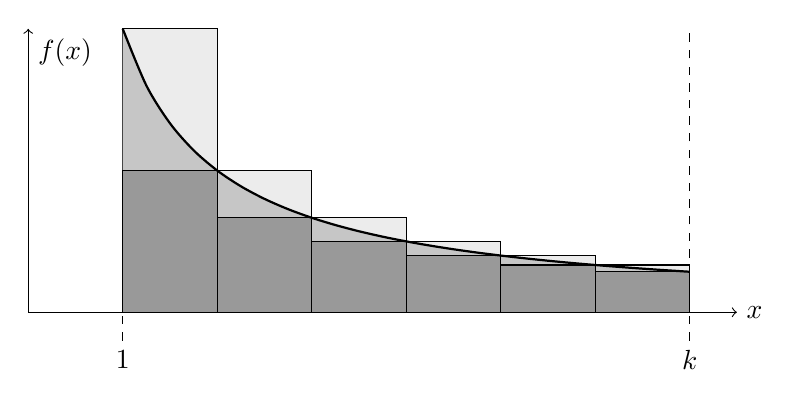
\begin{tikzpicture}[scale=1.2]
    \draw[->] (0,0) -- (7.5,0) node[right] {$x$};
    \draw[->] (0,0) -- (0,3) node[below right] {$f(x)$};

    \node[below] at (1,-0.3) {$1$};
    \draw[dashed] (1,-0.3) -- (1,3);
    \node[below] at (7,-0.3) {$k$};
    \draw[dashed] (7,-0.3) -- (7,3);

    \def\dx{1}
    \foreach \i in {0,1,2,3,4,5} {
      \pgfmathsetmacro{\xleft}{1 + \i*\dx}
      \pgfmathsetmacro{\height}{3/\xleft}
      \filldraw[fill=gray!15] (\xleft,0) rectangle ({\xleft+\dx}, {\height});
    }
    \fill[fill=gray!45, domain=1:7, smooth, variable=\x] (1, 1) -- plot ({\x}, {3/\x}) -- (7, 0) -- (1, 0) -- cycle;
    \foreach \i in {0,1,2,3,4,5} {
      \pgfmathsetmacro{\xleft}{1 + \i*\dx}
      \pgfmathsetmacro{\height}{3/(\xleft + \dx)}
      \filldraw[fill=gray!80] (\xleft,0) rectangle ({\xleft+\dx}, {\height});
    }
    \draw[thick, domain=1:7, smooth, variable=\x] plot ({\x}, {3/\x});
  \end{tikzpicture}
  \end{center}
  then we arrive at the following inequality:
  \[
    \text{Area of dark grey rectangles} \leq \text{Area under curve} \leq \text{Area of light grey rectangles}
  \]
  Translating this into sums of $a_n$ and integrals, we have:
  \begin{equation}
    s_k - a_1 = \sum_{n = 2}^{k} a_n \leq \int_{1}^{k} f(t) \d{t} \leq \sum_{n = 1}^{k - 1} a_n = s_{k - 1} \tag{$\ast$} \label{eqnAst1}
  \end{equation}
  Since $a_n \geq 0\ \forall n$, the partial sums $s_k$ must be monotonically increasing.
  \begin{proofdirection}{Assume series converges}
    As the series converges, we must have $s_k \to s$ for some finite $s$.
    Since $(s_k)$ is increasing, we must have $s_k \leq s\ \forall k$.
    We can then use \cref{eqnAst1} to bound the integral as $\int_{1}^{k} f(t) \d{t} \leq s_{k - 1} \leq s$.
    Thus, $(\int_{1}^{k} f(t) \d{t})_{k \in \N}$ is an increasing bounded sequence and so by the monotone convergence theorem (\cref{monotoneConvergence}), it converges.
  \end{proofdirection}
  \begin{proofdirection}{Assume integral converges}
    As the limit of the integral exists, by \cref{convergenceBounded}, the sequence $(\int_{1}^{k} f(t) \d{t})_k$ is bounded, hence $s_k$ is also bounded as $s_k \leq (\int_{1}^{k} f(t) \d{t}) + a_1$ from \cref{eqnAst1}.
    We also know that $(s_k)$ is increasing and so must converge by the monotone convergence theorem (\cref{monotoneConvergence}).
  \end{proofdirection}\par
  \textbf{Difference Between Sum and Integral}\par
  For the limit of the difference between the sum and the integral, set $b_k = \sum_{n = 1}^{k} a_n - \int_{1}^{k} f(t) \d{t}$.
  We then have:
  \[
    b_k - b_{k - 1} = a_k - \int_{k - 1}^{k} f(t) \d{t} = f(k) - \int_{k - 1}^{k} f(t) \d{t}
  \]
  For a decreasing function, we can visually see that $\int_{k - 1}^{k} f(t) \d{t} \geq \int_{k-1}^{k} f(k) \d{t} = f(k)$.
  So $b_k - b_{k - 1} \leq 0 \implies b_k \leq b_{k - 1}$ and so $(b_k)$ is decreasing.
  Furthermore, from the right inequality of \cref{eqnAst1}:
  \begin{align*}
    \sum_{n = 1}^{k - 1} a_n - \int_{1}^{k} f(t) \d{t} &\geq 0 \\
    \implies b_k = \sum_{n = 1}^{k} a_n - \int_{1}^{k} f(t) \d{t} &\geq a_k
  \end{align*}
  So $b_k \geq a_k = f(k) \geq 0$.
  Thus $(b_k)$ is bounded below by 0 so using the monotone convergence theorem, it converges to a limit $\ell$.

  Using the left inequality of \cref{eqnAst1}:
  \begin{align*}
    \sum_{n = 2}^{k} a_n - \int_{1}^{k} f(t) \d{t} &\leq 0 \\
    \implies b_k = \sum_{n = 1}^{k} a_n - \int_{1}^{k} f(t) \d{t} &\leq a_n
  \end{align*}
  Therefore, $0 \leq b_k \leq a_1$ so as we take the limit, the non strict inequalities are preserved by \cref{sandwichThm} so $0 \leq \ell \leq a_1$.
\end{proof}
\begin{remark}
  \begin{enumerate}
    \item $\lim_{n \to \infty} \int_{1}^{n} f(t) \d{t}$ is a type of \textit{improper integral}, these will be covered later in the course.
    \item The limit of the difference between the integral and the sum being so well bounded tells us that the integral is quite sharp in estimating the sum of the series if it converges, or the rate of divergence if it diverges.
  \end{enumerate}
\end{remark}
\begin{example}
  \begin{enumerate}
    \item Consider the series $\sum_{n = 1}^{\infty} \frac{1}{n^{p}}$ for $p \in \R$.

      Let $f(t) = t^{p}$, this is decreasing and continuous on $[1, \infty)$ and $f(t) \geq 0\ \forall t$ so we can apply the integral test.
      \[
        \lim_{n \to \infty}  \int_{1}^{n} \frac{1}{t^{p}} \d{t} = \lim_{n \to \infty} \begin{cases}
        \log n & \text{ for $p = 1$} \\
        \frac{1}{p - 1}(1 - n^{-p + 1}) & \text{ for $p \neq 1$}
        \end{cases}
      \]
      For $p = 1$, $\log n$ diverges to $\infty$ as $n \to \infty$.
      For $p \neq 1$:
      \[
        \frac{1}{p - 1}(1 - n^{-p + 1}) \to \begin{cases}
          \frac{1}{p - 1} & p > 1 \\
          \text{diverges to } \infty & p < 1
        \end{cases}
      \]
      Thus, the integral converges if and only if $p > 1$ and so the series converges if and only if $p > 1$.
    \item Consider the series $\sum_{n = 2}^{\infty} \frac{1}{n \log n}$.
      Let $f(t) = \frac{1}{t \log t}$, this is decreasing and continuous on $[2, \infty)$ (note that the sum starts from 2) so we can use the integral test:
      \[
        \int_2^n \frac{1}{t \log t} \d{t} \stackrel{u = \log t} = \int_{\log 2}^{\log n} \frac{\d{u}}{u} = \eval{\log u}{\log 2}{\log n} = \log(\log n) - \log(\log(2)) \to \infty
      \]
      So the series must diverge.
    \item $\sum_{n = 2}^{\infty} \frac{1}{n \log^2 n}$ converges by the integral test.
      Let $f(t) = \frac{1}{t\log^2 t}$, this satisfies the requirements to use the integral test so consider:
      \[
        \int_2^n \frac{1}{t \log^2 t} \d{t} \stackrel{u = \log t} = \int_{\log 2}^{\log n} \frac{\d{u}}{u^2} = \eval{-\frac{1}{u}}{\log 2}{\log n} = \frac{1}{\log(2)} - \frac{1}{\log(n)} \to \frac{1}{\log(2)}
      \]
      So the series must converge.
  \end{enumerate}
\end{example}
\begin{proposition}[Cauchy Condensation Test]
  If $(a_n)$ is a decreasing sequence such that $a_n \geq 0\ \forall n$, then $\sum_{n = 1}^{\infty} a_n$ converges if and only if $\sum_{n = 1}^{\infty} 2^{n}a_{2^{n}}$ converges.
\end{proposition}
\begin{proof}
  Not lectured.
\end{proof}
\subsubsection{Alternating Series Test and Dirichlet Test}
What about sequences with with infinitely many negative terms?
\begin{proposition}[Alternating Series Test]
  If $(a_n)$ is a decreasing sequence where all of the terms are non-negative and $a_n \to 0$, then $\sum_{n = 1}^{\infty} (-1)^{n + 1}a_n$ converges.
\end{proposition}
\begin{proof}
  Set $s_k = \sum_{n = 1}^{k} (-1)^{n + 1} a_n$. Then, for the even subsequence:
  \[
    s_{2k} = \underbrace{(a_1 - a_2)}_{\geq0} + \underbrace{(a_3 - a_4)}_{\geq 0} + \cdots + \underbrace{(a_{2k - 1} - a_{2k})}_{\geq 0}
  \]
  Therefore, $s_2 \leq s_4 \leq \cdots$, that is, $(s_{2k})$ is increasing.
  We can do a similar thing with the odd subsequence:
  \[
    s_{2k + 1} = a_1 + \underbrace{(-a_2 + a_3)}_{\leq 0} + \underbrace{(-a_4 + a_5)}_{\leq 0} + \cdots \underbrace{(-a_{2k} + a_{2k + 1})}_{\leq 0}
  \]
  Therefore, $s_1 \geq s_3 \geq \cdots$, that is, $(s_{2k + 1})$ is decreasing.

  Moreover, $s_{2k + 1} - s_{2k} = a_{2k + 1} \geq 0$ so we can create a chain of inequalities:
  \[
    a_1 - a_2 = s_2 \leq s_{2k} \leq s_{2k + 1} \leq s_1 = a_1
  \]
  Therefore $(s_{2k})$ is upper bounded by $a_1$ and $(s_{2k + 1})$ is lower bounded by $a_1 - a_2$.
  Thus by monotone convergence theorem (\cref{monotoneConvergence}), both sequences converge.

  Let $s = \lim_{k \to \infty} s_{2k}$ and $\widetilde{s} = \lim_{k \to \infty} s_{2k + 1}$.
  Now note that since $a_n \to 0$, by \cref{subseqenceConvergence}, the subsequence $a_{2k + 1} \to 0$ as $k \to \infty$.
  Therefore:
  \[
    s - \widetilde{s} = \lim_{k \to \infty} (s_{2k} - s_{2k + 1}) = \lim_{k \to \infty} a_{2k + 1} = 0
  \]
  So the odd and even subsequences of $(s_k)$ converge to the same limit.
  Therefore, by \cref{evenOddSubseq}, $s_k \to s$ so the series converges.
\end{proof}
\begin{example}
  \label{absoluteConvergenceCE}
  We know that $\sum_{n = 1}^{\infty} \frac{1}{n}$ diverges, however, if we consider the series $\sum_{n = 1}^{\infty} \frac{(-1)^{n + 1}}{n}$, then by the alternating series test, this converges.
  In fact, it converges to $\log 2$.
\end{example}
\begin{proposition}[Dirichlet Test]
  If $(a_n)$ is a decreasing sequence where $a_n \geq 0\ \forall n$ and $a_n \to 0$ and $(b_n)$ is a sequence such that $(s_k = \sum_{n = 1}^{k} b_n)_k$ is a bounded sequence, then $\sum_{n = 1}^{\infty} a_n b_n$ converges.
\end{proposition}
\begin{proof}
  See Example Sheet 1 Q12.
\end{proof}
\begin{remark}
  This is a more general result than the alternating series test as we can use $(b_n)$ to introduce more complicated sign patterns.
\end{remark}
\subsection{Absolute Convergence}
\begin{definition}[Absolute Convergence]
  We say that the series $\sum_{n = 1}^{\infty} a_n$ is \textit{absolutely convergent} if $\sum_{n = 1}^{\infty} |a_n|$ converges.
\end{definition}
\begin{remark}
  Note that $|a_n| \geq 0\ \forall n$ so the convergence tests that require positive terms are useful for determining if a series is absolutely convergent.
\end{remark}
\begin{lemma}
  If a series is absolutely convergent, then the original series converges.
  \label{absoluteImpliesConvergence}
\end{lemma}
\begin{proof}
  Let $s_k = \sum_{n = 1}^{k} a_n$ and $r_k = \sum_{n = 1}^{k} |a_n|$.
  For all $k > l$:
  \begin{align*}
    |s_k - s_l| = \abs{\sum_{n = l + 1}^{k} a_n} \leq \sum_{n = l + 1}^{k} |a_n| = r_k - r_l
  \end{align*}
  as the triangle inequality extends to arbitrarily many terms.

  By assumption, the series is absolutely convergent so $(r_k)$ is convergent and, by \cref{convergenceCauchy}, it must also be Cauchy.
  Therefore, by the above inequality, $(s_k)$ is also Cauchy, and so by the completeness of $\R$ and $\C$ (\cref{completenessOfRC}), $(s_k)$ converges.
\end{proof}
\begin{remark}
  We see that the converse of the above is false using \cref{absoluteConvergenceCE} so absolute convergence is stronger than convergence.

  We sometimes call convergent sequences which are \textbf{not} absolutely convergent \textit{conditionally convergent}.
\end{remark}
\begin{example}[Rearranging a conditionally convergent series]
  Consider again the series $\sum_{n = 1}^{\infty} \frac{(-1)^{n + 1}}{n} = 1 - \frac{1}{2} + \frac{1}{3} - \frac{1}{4} + \frac{1}{5} - \cdots$.
  This is conditionally convergent as $\sum_{n = 1}^{\infty} |a_n|$ diverges but $\sum_{n = 1}^{\infty} a_n = \log 2$.

  We can rearrange the terms of the sum as:
  \begin{align*}
    &\left(1 - \frac{1}{2}\right) - \frac{1}{4} + \left(\frac{1}{3} - \frac{1}{6}\right) - \frac{1}{8} + \left(\frac{1}{5} - \frac{1}{10}\right) - \frac{1}{12} + \left(\frac{1}{7} - \frac{1}{14}\right) + \cdots \\
    &= \frac{1}{2} - \frac{1}{4} + \frac{1}{6} - \frac{1}{8} + \frac{1}{10} - \frac{1}{12} + \frac{1}{14} + \cdots \\
    &= \frac{1}{2}\left(1 - \frac{1}{2} + \frac{1}{3} - \frac{1}{4} + \frac{1}{5} - \frac{1}{6} + \cdots\right) \\
    &= \frac{1}{2}\sum_{n = 1}^{\infty} \frac{(-1)^{n + 1}}{n}
  \end{align*}
  This seems to suggest that $\sum_{n = 1}^{\infty} \frac{(-1)^{n + 1}}{n} = \frac{1}{2} \sum_{n = 1}^{\infty} \frac{(-1)^{n + 1}}{n}$ which is clearly \textbf{not true}.

  If you have a conditionally convergent series, \textbf{the order of the sum matters}.
  This is not the case for absolutely convergent series.
\end{example}
\begin{proposition}[Rearrangements under absolute convergence]
  Let $\sigma: \N \to \N$ be a bijection (i.e. a permutation of $\N$) so that $a_n' = a_{\sigma(n)}$ is the rearranged sequence.
  If $\sum_{n = 1}^{\infty} a_n$ is absolutely convergent, then $\sum_{n = 1}^{\infty} a_n = \sum_{n = 1}^{\infty} a_n'$.
\end{proposition}
\begin{proof}
  Let $s_k = \sum_{n = 1}^{k} a_n$, $r_k = \sum_{n = 1}^{k} a_n'$ and $t_k = \sum_{n = 1}^{k} |a_n|$.
  Since the series is absolutely convergent, $t_k \to t$ as $k \to \infty$.
  Furthermore, by \cref{absoluteImpliesConvergence}, since it is absolutely convergent, the original series converges so $s_k \to s$ as $k \to \infty$.

  Therefore, $\forall \varepsilon > 0$:
  \begin{align*}
    \exists N_1 \text{ s.t. } |s_k - s| &< \varepsilon\ \forall k \geq N_1 \\
    \exists N_2 \text{ s.t. } |t_k - t| &< \varepsilon\ \forall k \geq N_2
  \end{align*}
  For $k \geq N_2$, we have:
  \[
    |t_k - t| = \sum_{n = 1}^{\infty} |a_n| - \sum_{n = 1}^{k} |a_n| = \sum_{n = k + 1}^{\infty} |a_n| < \varepsilon
  \]
  Note that we were able to subtract the first $k$ terms without affecting convergence by \cref{seriesTail}.
  Taking $k = N_2$, we have $\sum_{n = N_2 + 1}^{\infty} |a_n| < \varepsilon$.
  So, if we take $N = \max\{N_1, N_2\} + 1$, then $\sum_{n = N}^{\infty} |a_n| < \varepsilon$ and $|s_N - s| < \varepsilon$.

  The sequence terms $a_1, \ldots, a_N$ are mapped to $a_{\sigma(1)}, \ldots, a_{\sigma(N)}$ under the rearrangement.
  If we let $M = \max\{\sigma(1), \ldots, \sigma(N)\}$ then $a_1, \ldots, a_N$ must all be included in $a_1', \cdots, a_{M}'$ and the terms which are not from $a_1, \ldots, a_N$ must all have index $\geq N$ in the original series.
  We must also have $M \geq N$ as it is the maximum of $N$ natural numbers.
  Hence for $m \geq M \geq N$:
  \begin{align*}
    r_m = \sum_{n = 1}^{m} a_n' &= \underbrace{\sum_{n = 1}^{N} a_n}_{s_N} + (m - N \text{ terms of $(a_n)$ sequence with $n \geq N$}) \\
    \implies r_m - s &= s_N - s + (m - N \text{ terms of $(a_n)$ sequence with $n \geq N$}) \\
    \implies |r_m - s| &\leq |s_N - s| + (m - N \text{ terms of $(|a_n|)$ sequence with $n \geq N$}) \\
                       &\leq |s_N - s| + \sum_{n = N}^{\infty} |a_n| \text{ as $|a_n| \geq 0\ \forall n$}\\
                       &< \varepsilon + \varepsilon = 2\varepsilon
  \end{align*}
  Hence partial sums $(r_k)$ of the rearranged series converge to the value of the original series, and so the rearranged series and the original series converge to the same value.
\end{proof}
\end{document}
